\PassOptionsToPackage{unicode=true}{hyperref} % options for packages loaded elsewhere
\PassOptionsToPackage{hyphens}{url}
%
\documentclass[]{article}
\usepackage{lmodern}
\usepackage{amssymb,amsmath}
\usepackage{ifxetex,ifluatex}
\usepackage{fixltx2e} % provides \textsubscript
\ifnum 0\ifxetex 1\fi\ifluatex 1\fi=0 % if pdftex
  \usepackage[T1]{fontenc}
  \usepackage[utf8]{inputenc}
  \usepackage{textcomp} % provides euro and other symbols
\else % if luatex or xelatex
  \usepackage{unicode-math}
  \defaultfontfeatures{Ligatures=TeX,Scale=MatchLowercase}
\fi
% use upquote if available, for straight quotes in verbatim environments
\IfFileExists{upquote.sty}{\usepackage{upquote}}{}
% use microtype if available
\IfFileExists{microtype.sty}{%
\usepackage[]{microtype}
\UseMicrotypeSet[protrusion]{basicmath} % disable protrusion for tt fonts
}{}
\IfFileExists{parskip.sty}{%
\usepackage{parskip}
}{% else
\setlength{\parindent}{0pt}
\setlength{\parskip}{6pt plus 2pt minus 1pt}
}
\usepackage{hyperref}
\hypersetup{
            pdftitle={OneMap Hidden Markov Model parallelization},
            pdfauthor={Cristiane Hayumi Taniguti   from Statistical Genetics Lab   Department of Genetics   Luiz de Queiroz College of Agriculture   University of São Paulo},
            pdfborder={0 0 0},
            breaklinks=true}
\urlstyle{same}  % don't use monospace font for urls
\usepackage[margin=1in]{geometry}
\usepackage{color}
\usepackage{fancyvrb}
\newcommand{\VerbBar}{|}
\newcommand{\VERB}{\Verb[commandchars=\\\{\}]}
\DefineVerbatimEnvironment{Highlighting}{Verbatim}{commandchars=\\\{\}}
% Add ',fontsize=\small' for more characters per line
\usepackage{framed}
\definecolor{shadecolor}{RGB}{248,248,248}
\newenvironment{Shaded}{\begin{snugshade}}{\end{snugshade}}
\newcommand{\AlertTok}[1]{\textcolor[rgb]{0.94,0.16,0.16}{#1}}
\newcommand{\AnnotationTok}[1]{\textcolor[rgb]{0.56,0.35,0.01}{\textbf{\textit{#1}}}}
\newcommand{\AttributeTok}[1]{\textcolor[rgb]{0.77,0.63,0.00}{#1}}
\newcommand{\BaseNTok}[1]{\textcolor[rgb]{0.00,0.00,0.81}{#1}}
\newcommand{\BuiltInTok}[1]{#1}
\newcommand{\CharTok}[1]{\textcolor[rgb]{0.31,0.60,0.02}{#1}}
\newcommand{\CommentTok}[1]{\textcolor[rgb]{0.56,0.35,0.01}{\textit{#1}}}
\newcommand{\CommentVarTok}[1]{\textcolor[rgb]{0.56,0.35,0.01}{\textbf{\textit{#1}}}}
\newcommand{\ConstantTok}[1]{\textcolor[rgb]{0.00,0.00,0.00}{#1}}
\newcommand{\ControlFlowTok}[1]{\textcolor[rgb]{0.13,0.29,0.53}{\textbf{#1}}}
\newcommand{\DataTypeTok}[1]{\textcolor[rgb]{0.13,0.29,0.53}{#1}}
\newcommand{\DecValTok}[1]{\textcolor[rgb]{0.00,0.00,0.81}{#1}}
\newcommand{\DocumentationTok}[1]{\textcolor[rgb]{0.56,0.35,0.01}{\textbf{\textit{#1}}}}
\newcommand{\ErrorTok}[1]{\textcolor[rgb]{0.64,0.00,0.00}{\textbf{#1}}}
\newcommand{\ExtensionTok}[1]{#1}
\newcommand{\FloatTok}[1]{\textcolor[rgb]{0.00,0.00,0.81}{#1}}
\newcommand{\FunctionTok}[1]{\textcolor[rgb]{0.00,0.00,0.00}{#1}}
\newcommand{\ImportTok}[1]{#1}
\newcommand{\InformationTok}[1]{\textcolor[rgb]{0.56,0.35,0.01}{\textbf{\textit{#1}}}}
\newcommand{\KeywordTok}[1]{\textcolor[rgb]{0.13,0.29,0.53}{\textbf{#1}}}
\newcommand{\NormalTok}[1]{#1}
\newcommand{\OperatorTok}[1]{\textcolor[rgb]{0.81,0.36,0.00}{\textbf{#1}}}
\newcommand{\OtherTok}[1]{\textcolor[rgb]{0.56,0.35,0.01}{#1}}
\newcommand{\PreprocessorTok}[1]{\textcolor[rgb]{0.56,0.35,0.01}{\textit{#1}}}
\newcommand{\RegionMarkerTok}[1]{#1}
\newcommand{\SpecialCharTok}[1]{\textcolor[rgb]{0.00,0.00,0.00}{#1}}
\newcommand{\SpecialStringTok}[1]{\textcolor[rgb]{0.31,0.60,0.02}{#1}}
\newcommand{\StringTok}[1]{\textcolor[rgb]{0.31,0.60,0.02}{#1}}
\newcommand{\VariableTok}[1]{\textcolor[rgb]{0.00,0.00,0.00}{#1}}
\newcommand{\VerbatimStringTok}[1]{\textcolor[rgb]{0.31,0.60,0.02}{#1}}
\newcommand{\WarningTok}[1]{\textcolor[rgb]{0.56,0.35,0.01}{\textbf{\textit{#1}}}}
\usepackage{graphicx,grffile}
\makeatletter
\def\maxwidth{\ifdim\Gin@nat@width>\linewidth\linewidth\else\Gin@nat@width\fi}
\def\maxheight{\ifdim\Gin@nat@height>\textheight\textheight\else\Gin@nat@height\fi}
\makeatother
% Scale images if necessary, so that they will not overflow the page
% margins by default, and it is still possible to overwrite the defaults
% using explicit options in \includegraphics[width, height, ...]{}
\setkeys{Gin}{width=\maxwidth,height=\maxheight,keepaspectratio}
\setlength{\emergencystretch}{3em}  % prevent overfull lines
\providecommand{\tightlist}{%
  \setlength{\itemsep}{0pt}\setlength{\parskip}{0pt}}
\setcounter{secnumdepth}{0}
% Redefines (sub)paragraphs to behave more like sections
\ifx\paragraph\undefined\else
\let\oldparagraph\paragraph
\renewcommand{\paragraph}[1]{\oldparagraph{#1}\mbox{}}
\fi
\ifx\subparagraph\undefined\else
\let\oldsubparagraph\subparagraph
\renewcommand{\subparagraph}[1]{\oldsubparagraph{#1}\mbox{}}
\fi

% set default figure placement to htbp
\makeatletter
\def\fps@figure{htbp}
\makeatother

\usepackage{etoolbox}
\makeatletter
\providecommand{\subtitle}[1]{% add subtitle to \maketitle
  \apptocmd{\@title}{\par {\large #1 \par}}{}{}
}
\makeatother
% https://github.com/rstudio/rmarkdown/issues/337
\let\rmarkdownfootnote\footnote%
\def\footnote{\protect\rmarkdownfootnote}

% https://github.com/rstudio/rmarkdown/pull/252
\usepackage{titling}
\setlength{\droptitle}{-2em}

\pretitle{\vspace{\droptitle}\centering\huge}
\posttitle{\par}

\preauthor{\centering\large\emph}
\postauthor{\par}

\predate{\centering\large\emph}
\postdate{\par}

\title{OneMap Hidden Markov Model parallelization}
\author{Cristiane Hayumi Taniguti from Statistical Genetics Lab Department of
Genetics Luiz de Queiroz College of Agriculture University of São Paulo}
\date{}

\begin{document}
\maketitle

The goal here is to optimize the speed of OneMap Hidden Markov Model
(HMM) (Margarido et al., 2007) algorithm to genetic distance estimation.
For this, we implemented in OneMap two approaches: \texttt{parmap}
function and the approach proposed in BatchMap package (Schiffthaler et
al., 2017), a fork from OneMap.

The \texttt{parmap} splits an ordered sequence into groups according to
the number of cores available to the analyses. The groups have an
overlap of markers in their edges, to be possible the later joint of
them. Here we use these overlap markers also to compare the estimated
genetic distance between groups and see how the process can affect the
maps distances.

The approach implemented in BatchMap (and now in OneMap) also divides
the sequence into batches, but the parallelization is limited by the
number of possible phases. Therefore, a maximum of four cores can be
used to estimate genetic distances for outcrossing species.

To be a fair comparison, here we use four cores for both approaches.

Tests:

All scenarios have 1 chromosome with 100 cM, 5 family F1, progeny size
of 150 individuals, 504 markers, 6 cores, and overlap of 5 markers.

\begin{itemize}
\tightlist
\item
  \textbf{Scenario 1}: 28 markers of each one of the 18 possible types,
  without missing data
\item
  \textbf{Scenario 2}: 168 markers of D1.10, D2.15, and B3.7 types,
  without missing data
\item
  \textbf{Scenario 3}: 28 markers of each one of the 18 possible types,
  25\% of missing data
\item
  \textbf{Scenario 4}: 168 markers of D1.10, D2.15 and B3.7 types, 25\%
  of missing data
\end{itemize}

Measures:

\begin{itemize}
\tightlist
\item
  Total size
\item
  Recombination fraction difference between overlap markers
\item
  Time to run
\end{itemize}

Another test applied was to increase the tolerance value of the HMM. All
scenarios were repeated with tolerance value of \(10^{-3}\) (the default
value is \(10^{-5}\)).

\hypertarget{packages}{%
\subsection{Packages}\label{packages}}

\begin{Shaded}
\begin{Highlighting}[]
\KeywordTok{library}\NormalTok{(parallel)}
\KeywordTok{library}\NormalTok{(onemap) }\CommentTok{# Since version 2.2.0}
\KeywordTok{library}\NormalTok{(tidyverse)}
\end{Highlighting}
\end{Shaded}

\hypertarget{functions}{%
\subsection{Functions}\label{functions}}

\begin{Shaded}
\begin{Highlighting}[]
\NormalTok{runcomp <-}\StringTok{ }\ControlFlowTok{function}\NormalTok{(n.marker, mk.types, n.types, miss.perc,}\DataTypeTok{tol=}\FloatTok{10E-5}\NormalTok{)\{}
\NormalTok{  n.fam <-}\StringTok{ }\DecValTok{5}
\NormalTok{  int.tot.size <-}\StringTok{ }\NormalTok{par.tot.size <-}\StringTok{ }\NormalTok{int.time <-}\StringTok{ }\KeywordTok{vector}\NormalTok{()}
\NormalTok{  par.time <-}\StringTok{ }\NormalTok{int.cms <-}\StringTok{ }\NormalTok{par.cms <-}\StringTok{  }\NormalTok{diff2 <-}\StringTok{ }\KeywordTok{vector}\NormalTok{()}
\NormalTok{  batch.tot.size  <-}\StringTok{ }\NormalTok{batch.time <-}\StringTok{ }\NormalTok{batch.cms <-}\StringTok{ }\KeywordTok{vector}\NormalTok{() }
  \ControlFlowTok{for}\NormalTok{(w }\ControlFlowTok{in} \DecValTok{1}\OperatorTok{:}\NormalTok{n.fam)\{}
    \KeywordTok{run_pedsim}\NormalTok{(}\DataTypeTok{chromosome =} \KeywordTok{c}\NormalTok{(}\StringTok{"Chr1"}\NormalTok{), }\DataTypeTok{n.marker =}\NormalTok{ n.marker, }
               \DataTypeTok{tot.size.cm =} \KeywordTok{c}\NormalTok{(}\DecValTok{100}\NormalTok{), }\DataTypeTok{centromere =} \KeywordTok{c}\NormalTok{(}\DecValTok{50}\NormalTok{),}
               \DataTypeTok{n.ind =} \DecValTok{200}\NormalTok{, }\DataTypeTok{mk.types =}\NormalTok{ mk.types,}
               \DataTypeTok{n.types =}\NormalTok{ n.types, }\DataTypeTok{pop =} \StringTok{"F1"}\NormalTok{, }\DataTypeTok{path.pedsim =} \StringTok{"~/Programs/PedigreeSim/"}\NormalTok{,}
               \DataTypeTok{name.mapfile =} \StringTok{"mapfile.map"}\NormalTok{, }\DataTypeTok{name.founderfile=}\StringTok{"founderfile.gen"}\NormalTok{,}
               \DataTypeTok{name.chromfile=}\StringTok{"sim.chrom"}\NormalTok{, }\DataTypeTok{name.parfile=}\StringTok{"sim.par"}\NormalTok{,}
               \DataTypeTok{name.out=}\StringTok{"sim_out"}\NormalTok{)}
    
    \KeywordTok{pedsim2raw}\NormalTok{(}\DataTypeTok{cross=}\StringTok{"outcross"}\NormalTok{, }\DataTypeTok{genofile =} \StringTok{"sim_out_genotypes.dat"}\NormalTok{, }
               \DataTypeTok{parent1 =} \StringTok{"P1"}\NormalTok{, }\DataTypeTok{parent2 =} \StringTok{"P2"}\NormalTok{, }
               \DataTypeTok{out.file =} \StringTok{"sim_out.example1.raw"}\NormalTok{, }\DataTypeTok{miss.perc =}\NormalTok{ miss.perc)}
    
\NormalTok{    df <-}\StringTok{ }\KeywordTok{read_onemap}\NormalTok{(}\StringTok{"sim_out.example1.raw"}\NormalTok{)}
    
\NormalTok{    twopts <-}\StringTok{ }\KeywordTok{rf_2pts}\NormalTok{(df)}
    
\NormalTok{    seq1 <-}\StringTok{ }\KeywordTok{make_seq}\NormalTok{(twopts, }\StringTok{"all"}\NormalTok{)}
    
\NormalTok{    batch_size <-}\StringTok{ }\KeywordTok{pick_batch_sizes}\NormalTok{(}\DataTypeTok{input.seq =}\NormalTok{ seq1, }
                                   \DataTypeTok{size =} \DecValTok{80}\NormalTok{, }
                                   \DataTypeTok{overlap =} \DecValTok{30}\NormalTok{, }
                                   \DataTypeTok{around =} \DecValTok{10}\NormalTok{)}
    
\NormalTok{    batch.time <-}\StringTok{ }\KeywordTok{rbind}\NormalTok{(batch.time, }
                        \KeywordTok{system.time}\NormalTok{(batch.map <-}\StringTok{ }\KeywordTok{map_overlapping_batches}\NormalTok{(}\DataTypeTok{input.seq =}\NormalTok{ seq1,}
                                         \DataTypeTok{size =}\NormalTok{ batch_size,}
                                         \DataTypeTok{phase_cores =} \DecValTok{4}\NormalTok{,}
                                         \DataTypeTok{overlap =} \DecValTok{30}\NormalTok{, }\DataTypeTok{rm_unlinked =}\NormalTok{ T)))}
    
\NormalTok{    batch.cms <-}\StringTok{ }\KeywordTok{rbind}\NormalTok{(batch.cms, }\KeywordTok{cumsum}\NormalTok{(}\KeywordTok{c}\NormalTok{(}\DecValTok{0}\NormalTok{, }\KeywordTok{haldane}\NormalTok{(batch.map[[}\DecValTok{1}\NormalTok{]]}\OperatorTok{$}\NormalTok{seq.rf))))}
\NormalTok{    batch.tot.size <-}\StringTok{ }\KeywordTok{c}\NormalTok{(batch.tot.size, batch.cms[}\KeywordTok{length}\NormalTok{(batch.cms)])}
    
\NormalTok{    int.time <-}\StringTok{ }\KeywordTok{rbind}\NormalTok{(int.time, }\KeywordTok{system.time}\NormalTok{(int.map <-}\StringTok{ }\KeywordTok{map}\NormalTok{(seq1, }\DataTypeTok{tol=}\NormalTok{tol)))}
\NormalTok{    int.cms <-}\StringTok{ }\KeywordTok{rbind}\NormalTok{(int.cms, }\KeywordTok{cumsum}\NormalTok{(}\KeywordTok{c}\NormalTok{(}\DecValTok{0}\NormalTok{,}\KeywordTok{haldane}\NormalTok{(int.map}\OperatorTok{$}\NormalTok{seq.rf))))}
\NormalTok{    int.tot.size <-}\StringTok{ }\KeywordTok{c}\NormalTok{(int.tot.size, int.cms[}\KeywordTok{length}\NormalTok{(int.cms)])}

\NormalTok{    par.time <-}\StringTok{ }\KeywordTok{rbind}\NormalTok{(par.time, }
                      \KeywordTok{system.time}\NormalTok{(map2 <-}\StringTok{ }\KeywordTok{parmap}\NormalTok{(}\DataTypeTok{input.seq =}\NormalTok{ seq1, }
                                                 \DataTypeTok{cores =} \DecValTok{6}\NormalTok{, }\DataTypeTok{overlap =} \DecValTok{5}\NormalTok{, }\DataTypeTok{tol=}\NormalTok{tol)))}

\NormalTok{    diff2 <-}\StringTok{ }\KeywordTok{rbind}\NormalTok{(diff2, map2[[}\DecValTok{1}\NormalTok{]])}

\NormalTok{    par.map <-}\StringTok{ }\NormalTok{map2[[}\DecValTok{2}\NormalTok{]]}
\NormalTok{    par.cms <-}\StringTok{ }\KeywordTok{rbind}\NormalTok{(par.cms, }\KeywordTok{cumsum}\NormalTok{(}\KeywordTok{c}\NormalTok{(}\DecValTok{0}\NormalTok{,}\KeywordTok{haldane}\NormalTok{(par.map}\OperatorTok{$}\NormalTok{seq.rf))))}
\NormalTok{    par.tot.size <-}\StringTok{ }\KeywordTok{c}\NormalTok{(par.tot.size, par.cms[}\KeywordTok{length}\NormalTok{(par.cms)])}
\NormalTok{  \}}
\NormalTok{  result <-}\StringTok{ }\KeywordTok{list}\NormalTok{(diff2, int.tot.size, par.tot.size, batch.tot.size, }
\NormalTok{                 int.time, par.time, batch.time, int.cms, par.cms, batch.cms)}
  \KeywordTok{names}\NormalTok{(result) <-}\StringTok{ }\KeywordTok{c}\NormalTok{(}\StringTok{"diff"}\NormalTok{, }\StringTok{"int.tot.size"}\NormalTok{, }\StringTok{"par.tot.size"}\NormalTok{, }
                     \StringTok{"batch.tot.size"}\NormalTok{, }\StringTok{"int.time"}\NormalTok{, }\StringTok{"par.time"}\NormalTok{, }
                     \StringTok{"batch.time"}\NormalTok{, }\StringTok{"int.cms"}\NormalTok{, }\StringTok{"par.cms"}\NormalTok{, }\StringTok{"batch.cms"}\NormalTok{)}
  
  \KeywordTok{return}\NormalTok{(result)}
\NormalTok{\}}
\end{Highlighting}
\end{Shaded}

\hypertarget{running-each-scenario}{%
\section{Running each scenario}\label{running-each-scenario}}

\begin{itemize}
\tightlist
\item
  scenario (1)
\end{itemize}

\begin{Shaded}
\begin{Highlighting}[]
\NormalTok{cen1 <-}\StringTok{ }\KeywordTok{runcomp}\NormalTok{(}\DataTypeTok{n.marker =} \DecValTok{504}\NormalTok{, }
                \DataTypeTok{mk.types =} \KeywordTok{c}\NormalTok{(}\StringTok{"A1"}\NormalTok{, }\StringTok{"A2"}\NormalTok{, }\StringTok{"A3"}\NormalTok{, }\StringTok{"A4"}\NormalTok{, }\StringTok{"B1.5"}\NormalTok{, }\StringTok{"B2.6"}\NormalTok{, }\StringTok{"B3.7"}\NormalTok{,}
                             \StringTok{"C.8"}\NormalTok{, }\StringTok{"D1.9"}\NormalTok{, }\StringTok{"D1.10"}\NormalTok{, }\StringTok{"D1.11"}\NormalTok{, }\StringTok{"D1.12"}\NormalTok{, }\StringTok{"D1.13"}\NormalTok{,}
                             \StringTok{"D2.14"}\NormalTok{, }\StringTok{"D2.15"}\NormalTok{, }\StringTok{"D2.16"}\NormalTok{, }\StringTok{"D2.17"}\NormalTok{, }\StringTok{"D2.18"}\NormalTok{),}
                \DataTypeTok{n.types =} \KeywordTok{rep}\NormalTok{(}\DecValTok{28}\NormalTok{,}\DecValTok{18}\NormalTok{),}
                \DataTypeTok{miss.perc =} \DecValTok{0}\NormalTok{)}
\end{Highlighting}
\end{Shaded}

\begin{itemize}
\tightlist
\item
  scenario (2)
\end{itemize}

\begin{Shaded}
\begin{Highlighting}[]
\NormalTok{cen2 <-}\StringTok{ }\KeywordTok{runcomp}\NormalTok{(}\DataTypeTok{n.marker =} \DecValTok{504}\NormalTok{, }
                \DataTypeTok{mk.types =} \KeywordTok{c}\NormalTok{(}\StringTok{"B3.7"}\NormalTok{,}\StringTok{"D1.10"}\NormalTok{, }\StringTok{"D2.15"}\NormalTok{),}
                \DataTypeTok{n.types =} \KeywordTok{rep}\NormalTok{(}\DecValTok{168}\NormalTok{,}\DecValTok{3}\NormalTok{),}
                \DataTypeTok{miss.perc =} \DecValTok{0}\NormalTok{)}
\end{Highlighting}
\end{Shaded}

\begin{itemize}
\tightlist
\item
  scenario (3)
\end{itemize}

\begin{Shaded}
\begin{Highlighting}[]
\NormalTok{cen3 <-}\StringTok{ }\KeywordTok{runcomp}\NormalTok{(}\DataTypeTok{n.marker =} \DecValTok{504}\NormalTok{, }
                \DataTypeTok{mk.types =} \KeywordTok{c}\NormalTok{(}\StringTok{"A1"}\NormalTok{, }\StringTok{"A2"}\NormalTok{, }\StringTok{"A3"}\NormalTok{, }\StringTok{"A4"}\NormalTok{, }\StringTok{"B1.5"}\NormalTok{, }\StringTok{"B2.6"}\NormalTok{, }\StringTok{"B3.7"}\NormalTok{,}
                             \StringTok{"C.8"}\NormalTok{, }\StringTok{"D1.9"}\NormalTok{, }\StringTok{"D1.10"}\NormalTok{, }\StringTok{"D1.11"}\NormalTok{, }\StringTok{"D1.12"}\NormalTok{, }\StringTok{"D1.13"}\NormalTok{,}
                             \StringTok{"D2.14"}\NormalTok{, }\StringTok{"D2.15"}\NormalTok{, }\StringTok{"D2.16"}\NormalTok{, }\StringTok{"D2.17"}\NormalTok{, }\StringTok{"D2.18"}\NormalTok{),}
                \DataTypeTok{n.types =} \KeywordTok{rep}\NormalTok{(}\DecValTok{28}\NormalTok{,}\DecValTok{18}\NormalTok{),}
                \DataTypeTok{miss.perc =} \DecValTok{25}\NormalTok{)}
\end{Highlighting}
\end{Shaded}

\begin{itemize}
\tightlist
\item
  scenario (4)
\end{itemize}

\begin{Shaded}
\begin{Highlighting}[]
\NormalTok{cen4 <-}\StringTok{ }\KeywordTok{runcomp}\NormalTok{(}\DataTypeTok{n.marker =} \DecValTok{504}\NormalTok{, }
                \DataTypeTok{mk.types =} \KeywordTok{c}\NormalTok{(}\StringTok{"B3.7"}\NormalTok{,}\StringTok{"D1.10"}\NormalTok{, }\StringTok{"D2.15"}\NormalTok{),}
                \DataTypeTok{n.types =} \KeywordTok{rep}\NormalTok{(}\DecValTok{168}\NormalTok{,}\DecValTok{3}\NormalTok{),}
                \DataTypeTok{miss.perc =} \DecValTok{25}\NormalTok{)}
\end{Highlighting}
\end{Shaded}

\begin{itemize}
\tightlist
\item
  scenario (1) tol
\end{itemize}

\begin{Shaded}
\begin{Highlighting}[]
\NormalTok{cen1.tol <-}\StringTok{ }\KeywordTok{runcomp}\NormalTok{(}\DataTypeTok{n.marker =} \DecValTok{504}\NormalTok{, }
                    \DataTypeTok{mk.types =} \KeywordTok{c}\NormalTok{(}\StringTok{"A1"}\NormalTok{, }\StringTok{"A2"}\NormalTok{, }\StringTok{"A3"}\NormalTok{, }\StringTok{"A4"}\NormalTok{, }\StringTok{"B1.5"}\NormalTok{, }\StringTok{"B2.6"}\NormalTok{, }\StringTok{"B3.7"}\NormalTok{,}
                                 \StringTok{"C.8"}\NormalTok{, }\StringTok{"D1.9"}\NormalTok{, }\StringTok{"D1.10"}\NormalTok{, }\StringTok{"D1.11"}\NormalTok{, }\StringTok{"D1.12"}\NormalTok{, }\StringTok{"D1.13"}\NormalTok{,}
                                 \StringTok{"D2.14"}\NormalTok{, }\StringTok{"D2.15"}\NormalTok{, }\StringTok{"D2.16"}\NormalTok{, }\StringTok{"D2.17"}\NormalTok{, }\StringTok{"D2.18"}\NormalTok{),}
                    \DataTypeTok{n.types =} \KeywordTok{rep}\NormalTok{(}\DecValTok{28}\NormalTok{,}\DecValTok{18}\NormalTok{),}
                    \DataTypeTok{miss.perc =} \DecValTok{0}\NormalTok{, }\DataTypeTok{tol=}\FloatTok{10E-4}\NormalTok{)}
\end{Highlighting}
\end{Shaded}

\begin{itemize}
\tightlist
\item
  scenario (2) tol
\end{itemize}

\begin{Shaded}
\begin{Highlighting}[]
\NormalTok{cen2.tol <-}\StringTok{ }\KeywordTok{runcomp}\NormalTok{(}\DataTypeTok{n.marker =} \DecValTok{504}\NormalTok{, }
                    \DataTypeTok{mk.types =} \KeywordTok{c}\NormalTok{(}\StringTok{"B3.7"}\NormalTok{,}\StringTok{"D1.10"}\NormalTok{, }\StringTok{"D2.15"}\NormalTok{),}
                    \DataTypeTok{n.types =} \KeywordTok{rep}\NormalTok{(}\DecValTok{168}\NormalTok{,}\DecValTok{3}\NormalTok{),}
                    \DataTypeTok{miss.perc =} \DecValTok{0}\NormalTok{, }\DataTypeTok{tol=}\FloatTok{10E-4}\NormalTok{)}
\end{Highlighting}
\end{Shaded}

\begin{itemize}
\tightlist
\item
  Scenario (3) tol
\end{itemize}

\begin{Shaded}
\begin{Highlighting}[]
\NormalTok{cen3.tol <-}\StringTok{ }\KeywordTok{runcomp}\NormalTok{(}\DataTypeTok{n.marker =} \DecValTok{504}\NormalTok{, }
                    \DataTypeTok{mk.types =} \KeywordTok{c}\NormalTok{(}\StringTok{"A1"}\NormalTok{, }\StringTok{"A2"}\NormalTok{, }\StringTok{"A3"}\NormalTok{, }\StringTok{"A4"}\NormalTok{, }\StringTok{"B1.5"}\NormalTok{, }\StringTok{"B2.6"}\NormalTok{, }\StringTok{"B3.7"}\NormalTok{,}
                                 \StringTok{"C.8"}\NormalTok{, }\StringTok{"D1.9"}\NormalTok{, }\StringTok{"D1.10"}\NormalTok{, }\StringTok{"D1.11"}\NormalTok{, }\StringTok{"D1.12"}\NormalTok{, }\StringTok{"D1.13"}\NormalTok{,}
                                 \StringTok{"D2.14"}\NormalTok{, }\StringTok{"D2.15"}\NormalTok{, }\StringTok{"D2.16"}\NormalTok{, }\StringTok{"D2.17"}\NormalTok{, }\StringTok{"D2.18"}\NormalTok{),}
                    \DataTypeTok{n.types =} \KeywordTok{rep}\NormalTok{(}\DecValTok{28}\NormalTok{,}\DecValTok{18}\NormalTok{),}
                    \DataTypeTok{miss.perc =} \DecValTok{25}\NormalTok{, }\DataTypeTok{tol=}\FloatTok{10E-4}\NormalTok{)}
\end{Highlighting}
\end{Shaded}

\begin{itemize}
\tightlist
\item
  Scenario (4) tol
\end{itemize}

\begin{Shaded}
\begin{Highlighting}[]
\NormalTok{cen4.tol <-}\StringTok{ }\KeywordTok{runcomp}\NormalTok{(}\DataTypeTok{n.marker =} \DecValTok{504}\NormalTok{, }
                    \DataTypeTok{mk.types =} \KeywordTok{c}\NormalTok{(}\StringTok{"B3.7"}\NormalTok{,}\StringTok{"D1.10"}\NormalTok{, }\StringTok{"D2.15"}\NormalTok{),}
                    \DataTypeTok{n.types =} \KeywordTok{rep}\NormalTok{(}\DecValTok{168}\NormalTok{,}\DecValTok{3}\NormalTok{),}
                    \DataTypeTok{miss.perc =} \DecValTok{25}\NormalTok{, }\DataTypeTok{tol=}\FloatTok{10E-4}\NormalTok{)}

\KeywordTok{save.image}\NormalTok{(}\StringTok{"results.RData"}\NormalTok{)}
\end{Highlighting}
\end{Shaded}

\hypertarget{results}{%
\section{Results}\label{results}}

Jointing information from all scenarios:

\begin{Shaded}
\begin{Highlighting}[]
\KeywordTok{load}\NormalTok{(}\StringTok{"results.RData"}\NormalTok{)}

\NormalTok{tot.size.cm <-}\StringTok{ }\DecValTok{100}
\NormalTok{n.marker <-}\StringTok{ }\DecValTok{504}
\NormalTok{int <-}\StringTok{ }\NormalTok{tot.size.cm}\OperatorTok{/}\NormalTok{n.marker}
\NormalTok{pos <-}\StringTok{ }\KeywordTok{seq}\NormalTok{(}\DataTypeTok{from=}\DecValTok{0}\NormalTok{, }\DataTypeTok{to=}\NormalTok{tot.size.cm, }\DataTypeTok{by=}\NormalTok{int)}

\NormalTok{tot.cen <-}\StringTok{ }\KeywordTok{list}\NormalTok{(cen1, cen1.tol, cen2.tol, cen2, cen3, cen3.tol, cen4, cen4.tol)}
\KeywordTok{names}\NormalTok{(tot.cen) <-}\StringTok{ }\KeywordTok{c}\NormalTok{(}\StringTok{"cen1"}\NormalTok{, }\StringTok{"cen1.tol"}\NormalTok{, }\StringTok{"cen2"}\NormalTok{, }\StringTok{"cen2.tol"}\NormalTok{, }
                    \StringTok{"cen3"}\NormalTok{, }\StringTok{"cen3.tol"}\NormalTok{, }\StringTok{"cen4"}\NormalTok{, }\StringTok{"cen4.tol"}\NormalTok{)}

\NormalTok{df_diff <-}\StringTok{ }\NormalTok{df_tot_size <-}\StringTok{ }\NormalTok{df_times <-}\StringTok{ }\NormalTok{df_sizes <-}\StringTok{  }\KeywordTok{vector}\NormalTok{()}
\ControlFlowTok{for}\NormalTok{(i }\ControlFlowTok{in} \DecValTok{1}\OperatorTok{:}\KeywordTok{length}\NormalTok{(tot.cen))\{}
  \CommentTok{# Diff}
\NormalTok{  temp.df <-}\StringTok{ }\KeywordTok{cbind}\NormalTok{(}\KeywordTok{paste0}\NormalTok{(}\StringTok{"simu"}\NormalTok{,}\DecValTok{1}\OperatorTok{:}\KeywordTok{length}\NormalTok{(tot.cen[[i]][[}\DecValTok{2}\NormalTok{]])), }
                   \KeywordTok{sqrt}\NormalTok{(tot.cen[[i]][[}\DecValTok{1}\NormalTok{]]}\OperatorTok{^}\DecValTok{2}\NormalTok{))}
  \KeywordTok{colnames}\NormalTok{(temp.df) <-}\StringTok{ }\KeywordTok{c}\NormalTok{(}\StringTok{"simu"}\NormalTok{, }\KeywordTok{paste0}\NormalTok{(}\StringTok{"Overlap"}\NormalTok{, }
                                        \DecValTok{1}\OperatorTok{:}\KeywordTok{dim}\NormalTok{(tot.cen[[i]][[}\DecValTok{1}\NormalTok{]])[}\DecValTok{2}\NormalTok{]))}
\NormalTok{  diff <-}\StringTok{ }\KeywordTok{gather}\NormalTok{(}\KeywordTok{data.frame}\NormalTok{(temp.df), key, value, }\OperatorTok{-}\NormalTok{simu)}
\NormalTok{  df_diff <-}\StringTok{ }\KeywordTok{rbind}\NormalTok{(df_diff, }\KeywordTok{data.frame}\NormalTok{(}\DataTypeTok{scen=} \KeywordTok{names}\NormalTok{(tot.cen)[i], diff))}
  
  \CommentTok{# tot.size}
\NormalTok{  temp.df <-}\StringTok{ }\KeywordTok{data.frame}\NormalTok{(tot.cen[[i]][}\KeywordTok{c}\NormalTok{(}\DecValTok{2}\OperatorTok{:}\DecValTok{3}\NormalTok{,}\DecValTok{8}\NormalTok{)]) }\CommentTok{# change here}
\NormalTok{  temp.df <-}\StringTok{ }\KeywordTok{cbind}\NormalTok{(}\DataTypeTok{simu =} \KeywordTok{paste0}\NormalTok{(}\StringTok{"simu"}\NormalTok{, }\DecValTok{1}\OperatorTok{:}\KeywordTok{length}\NormalTok{(tot.cen[[i]][[}\DecValTok{2}\NormalTok{]])), temp.df)}
  \KeywordTok{colnames}\NormalTok{(temp.df) <-}\StringTok{ }\KeywordTok{c}\NormalTok{(}\StringTok{"simu"}\NormalTok{, }\StringTok{"all"}\NormalTok{, }\StringTok{"parmap"}\NormalTok{, }\StringTok{"batchmap"}\NormalTok{)}
\NormalTok{  df_tot_size <-}\StringTok{ }\KeywordTok{rbind}\NormalTok{(df_tot_size, }\KeywordTok{data.frame}\NormalTok{(}\DataTypeTok{scen=} \KeywordTok{names}\NormalTok{(tot.cen)[i],temp.df))}
  
  \CommentTok{# time}
\NormalTok{  temp.df <-}\StringTok{ }\KeywordTok{data.frame}\NormalTok{(}\DataTypeTok{simu =} \KeywordTok{paste0}\NormalTok{(}\StringTok{"simu"}\NormalTok{, }\DecValTok{1}\OperatorTok{:}\KeywordTok{length}\NormalTok{(tot.cen[[i]][[}\DecValTok{2}\NormalTok{]])),}
                        \DataTypeTok{int.time=}\NormalTok{ tot.cen[[i]][[}\DecValTok{4}\NormalTok{]][,}\DecValTok{3}\NormalTok{], }
                        \DataTypeTok{par.time =}\NormalTok{ tot.cen[[i]][[}\DecValTok{5}\NormalTok{]][,}\DecValTok{3}\NormalTok{],}
                        \DataTypeTok{batch.time =}\NormalTok{ tot.cen[[i]][[}\DecValTok{9}\NormalTok{]][,}\DecValTok{3}\NormalTok{]) }\CommentTok{# change here}
  \KeywordTok{colnames}\NormalTok{(temp.df) <-}\StringTok{ }\KeywordTok{c}\NormalTok{(}\StringTok{"simu"}\NormalTok{, }\StringTok{"all"}\NormalTok{, }\StringTok{"parallel"}\NormalTok{, }\StringTok{"batchmap"}\NormalTok{)}
\NormalTok{  df_times <-}\StringTok{ }\KeywordTok{rbind}\NormalTok{(df_times, }\KeywordTok{data.frame}\NormalTok{(}\DataTypeTok{scen=} \KeywordTok{names}\NormalTok{(tot.cen)[i],temp.df))}
  
  
  \CommentTok{# cMs}
  
\NormalTok{  temp.int <-}\StringTok{ }\KeywordTok{t}\NormalTok{(}\KeywordTok{apply}\NormalTok{(tot.cen[[i]][[}\DecValTok{6}\NormalTok{]],}\DecValTok{1}\NormalTok{, }\ControlFlowTok{function}\NormalTok{(x) }\KeywordTok{sqrt}\NormalTok{((x}\OperatorTok{-}\NormalTok{pos[}\OperatorTok{-}\DecValTok{1}\NormalTok{])}\OperatorTok{^}\DecValTok{2}\NormalTok{)))}
\NormalTok{  temp.par <-}\StringTok{ }\KeywordTok{t}\NormalTok{(}\KeywordTok{apply}\NormalTok{(tot.cen[[i]][[}\DecValTok{7}\NormalTok{]],}\DecValTok{1}\NormalTok{, }\ControlFlowTok{function}\NormalTok{(x) }\KeywordTok{sqrt}\NormalTok{((x}\OperatorTok{-}\NormalTok{pos[}\OperatorTok{-}\DecValTok{1}\NormalTok{])}\OperatorTok{^}\DecValTok{2}\NormalTok{)))}
\NormalTok{  temp.batch <-}\StringTok{ }\KeywordTok{t}\NormalTok{(}\KeywordTok{apply}\NormalTok{(tot.cen[[i]][[}\DecValTok{10}\NormalTok{]],}\DecValTok{1}\NormalTok{, }\ControlFlowTok{function}\NormalTok{(x) }\KeywordTok{sqrt}\NormalTok{((x}\OperatorTok{-}\NormalTok{pos[}\OperatorTok{-}\DecValTok{1}\NormalTok{])}\OperatorTok{^}\DecValTok{2}\NormalTok{)))}
  
  \KeywordTok{colnames}\NormalTok{(temp.int) <-}\StringTok{ }\KeywordTok{paste0}\NormalTok{(}\StringTok{"MK"}\NormalTok{,}\DecValTok{1}\OperatorTok{:}\KeywordTok{dim}\NormalTok{(temp.int)[}\DecValTok{2}\NormalTok{])}
  \KeywordTok{colnames}\NormalTok{(temp.par) <-}\StringTok{ }\KeywordTok{paste0}\NormalTok{(}\StringTok{"MK"}\NormalTok{,}\DecValTok{1}\OperatorTok{:}\KeywordTok{dim}\NormalTok{(temp.par)[}\DecValTok{2}\NormalTok{])}
  \KeywordTok{colnames}\NormalTok{(temp.batch) <-}\StringTok{ }\KeywordTok{paste0}\NormalTok{(}\StringTok{"MK"}\NormalTok{,}\DecValTok{1}\OperatorTok{:}\KeywordTok{dim}\NormalTok{(temp.batch)[}\DecValTok{2}\NormalTok{])}
  
\NormalTok{  temp.int <-}\StringTok{ }\KeywordTok{data.frame}\NormalTok{(}\DataTypeTok{simu =} \KeywordTok{paste0}\NormalTok{(}\StringTok{"simu"}\NormalTok{, }\DecValTok{1}\OperatorTok{:}\KeywordTok{length}\NormalTok{(tot.cen[[i]][[}\DecValTok{2}\NormalTok{]])),}
\NormalTok{                         temp.int)}
\NormalTok{  temp.int <-}\StringTok{ }\KeywordTok{gather}\NormalTok{(temp.int, key, value,}\OperatorTok{-}\NormalTok{simu)}
\NormalTok{  temp.par <-}\StringTok{ }\KeywordTok{data.frame}\NormalTok{(}\DataTypeTok{simu =} \KeywordTok{paste0}\NormalTok{(}\StringTok{"simu"}\NormalTok{, }\DecValTok{1}\OperatorTok{:}\KeywordTok{length}\NormalTok{(tot.cen[[i]][[}\DecValTok{2}\NormalTok{]])),}
\NormalTok{                         temp.par)}
\NormalTok{  temp.par <-}\StringTok{ }\KeywordTok{gather}\NormalTok{(temp.par, key, value,}\OperatorTok{-}\NormalTok{simu)}
\NormalTok{  temp.batch <-}\StringTok{ }\KeywordTok{data.frame}\NormalTok{(}\DataTypeTok{simu =} \KeywordTok{paste0}\NormalTok{(}\StringTok{"simu"}\NormalTok{, }\DecValTok{1}\OperatorTok{:}\KeywordTok{length}\NormalTok{(tot.cen[[i]][[}\DecValTok{2}\NormalTok{]])),}
\NormalTok{                         temp.batch)}
\NormalTok{  temp.batch <-}\StringTok{ }\KeywordTok{gather}\NormalTok{(temp.batch, key, value,}\OperatorTok{-}\NormalTok{simu)}
  
\NormalTok{  temp.df <-}\StringTok{ }\KeywordTok{merge}\NormalTok{(temp.int, temp.par, }\DataTypeTok{by =} \KeywordTok{c}\NormalTok{(}\StringTok{"simu"}\NormalTok{, }\StringTok{"key"}\NormalTok{))}
\NormalTok{  temp.df <-}\StringTok{ }\KeywordTok{merge}\NormalTok{(temp.df, temp.batch, }\DataTypeTok{by=}\KeywordTok{c}\NormalTok{(}\StringTok{"simu"}\NormalTok{, }\StringTok{"key"}\NormalTok{))}
  \KeywordTok{colnames}\NormalTok{(temp.df) <-}\StringTok{ }\KeywordTok{c}\NormalTok{(}\StringTok{"simu"}\NormalTok{, }\StringTok{"mk"}\NormalTok{, }\StringTok{"all"}\NormalTok{, }\StringTok{"parmap"}\NormalTok{, }\StringTok{"batchmap"}\NormalTok{)}
\NormalTok{  df_sizes <-}\StringTok{ }\KeywordTok{rbind}\NormalTok{(df_sizes, }\KeywordTok{data.frame}\NormalTok{(}\DataTypeTok{scen =} \KeywordTok{names}\NormalTok{(tot.cen)[i],temp.df))}
\NormalTok{\}}
\end{Highlighting}
\end{Shaded}

\hypertarget{time}{%
\subsection{Time}\label{time}}

Comparison between time spent for each approach: BatchMap, parmap, and
OneMap without parallelization (map function).

\begin{Shaded}
\begin{Highlighting}[]
\CommentTok{# rename columns}
\KeywordTok{colnames}\NormalTok{(df_times)[}\DecValTok{3}\OperatorTok{:}\DecValTok{5}\NormalTok{] <-}\StringTok{ }\KeywordTok{c}\NormalTok{(}\StringTok{"without parallel"}\NormalTok{, }\StringTok{"parmap"}\NormalTok{, }\StringTok{"BatchMap"}\NormalTok{)}

\NormalTok{df_times }\OperatorTok\StringTok{ }\KeywordTok{gather}\NormalTok{(key, value, }\OperatorTok{-}\NormalTok{simu, }\OperatorTok{-}\NormalTok{scen) }\OperatorTok
\StringTok{  }\KeywordTok{ggplot}\NormalTok{(}\KeywordTok{aes}\NormalTok{(}\DataTypeTok{x=}\NormalTok{scen, }\DataTypeTok{y=}\NormalTok{value}\OperatorTok{/}\DecValTok{3600}\NormalTok{, }\DataTypeTok{color=}\NormalTok{key)) }\OperatorTok{+}\StringTok{ }
\StringTok{  }\KeywordTok{geom_boxplot}\NormalTok{() }\OperatorTok{+}
\StringTok{  }\KeywordTok{xlab}\NormalTok{(}\StringTok{"scenarios"}\NormalTok{) }\OperatorTok{+}\StringTok{ }
\StringTok{  }\KeywordTok{ylab}\NormalTok{(}\StringTok{"Time (hours)"}\NormalTok{) }\OperatorTok{+}
\StringTok{  }\KeywordTok{scale_color_discrete}\NormalTok{(}\DataTypeTok{name=}\StringTok{"method"}\NormalTok{)}
\end{Highlighting}
\end{Shaded}

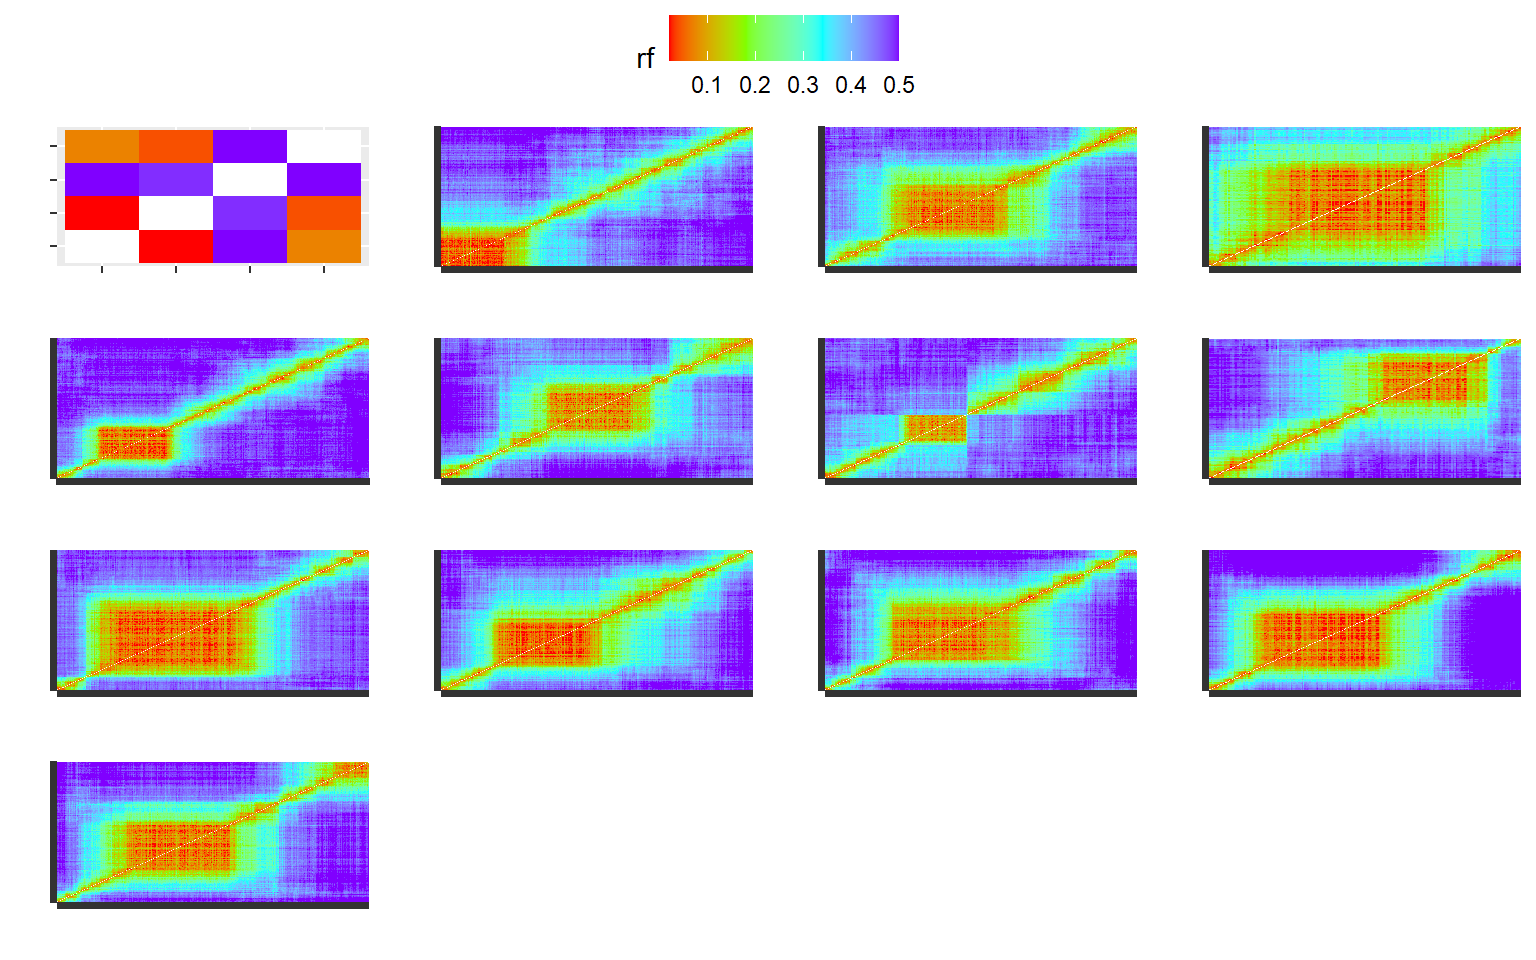
\includegraphics{Parallel_HMM_pdf_files/figure-latex/unnamed-chunk-12-1.pdf}

\hypertarget{total-sizes}{%
\subsection{Total sizes}\label{total-sizes}}

Comparison between total map size built by each approach: BatchMap,
parmap, and OneMap without parallelization (map function). Remember here
that the simulated size was 100 cM (red line).

\begin{Shaded}
\begin{Highlighting}[]
\CommentTok{# rename columns}
\KeywordTok{colnames}\NormalTok{(df_tot_size)[}\DecValTok{3}\OperatorTok{:}\DecValTok{5}\NormalTok{] <-}\StringTok{ }\KeywordTok{c}\NormalTok{(}\StringTok{"without parallel"}\NormalTok{, }\StringTok{"parmap"}\NormalTok{, }\StringTok{"BatchMap"}\NormalTok{)}

\NormalTok{df_tot_size }\OperatorTok\StringTok{ }\KeywordTok{gather}\NormalTok{(key, value, }\OperatorTok{-}\NormalTok{scen, }\OperatorTok{-}\NormalTok{simu) }\OperatorTok
\StringTok{  }\KeywordTok{ggplot}\NormalTok{(}\KeywordTok{aes}\NormalTok{(}\DataTypeTok{x=}\NormalTok{scen, }\DataTypeTok{y=}\NormalTok{value, }\DataTypeTok{color=}\NormalTok{key)) }\OperatorTok{+}
\StringTok{  }\KeywordTok{geom_boxplot}\NormalTok{() }\OperatorTok{+}\StringTok{ }
\StringTok{  }\KeywordTok{geom_hline}\NormalTok{(}\DataTypeTok{yintercept=}\DecValTok{100}\NormalTok{, }\DataTypeTok{color =} \StringTok{"red"}\NormalTok{) }\OperatorTok{+}
\StringTok{  }\KeywordTok{theme}\NormalTok{(}\DataTypeTok{axis.text.x =} \KeywordTok{element_text}\NormalTok{(}\DataTypeTok{angle =} \DecValTok{70}\NormalTok{, }\DataTypeTok{hjust =} \DecValTok{1}\NormalTok{)) }\OperatorTok{+}
\StringTok{  }\KeywordTok{xlab}\NormalTok{(}\StringTok{"scenarios"}\NormalTok{) }\OperatorTok{+}\StringTok{ }
\StringTok{  }\KeywordTok{ylab}\NormalTok{(}\StringTok{"Difference between total size (cM)"}\NormalTok{) }\OperatorTok{+}
\StringTok{  }\KeywordTok{scale_color_discrete}\NormalTok{(}\DataTypeTok{name=}\StringTok{"method"}\NormalTok{) }\OperatorTok{+}
\StringTok{  }\KeywordTok{expand_limits}\NormalTok{(}\DataTypeTok{x =} \DecValTok{0}\NormalTok{, }\DataTypeTok{y =} \DecValTok{0}\NormalTok{)}
\end{Highlighting}
\end{Shaded}

\includegraphics{Parallel_HMM_pdf_files/figure-latex/unnamed-chunk-13-1.pdf}

\hypertarget{intervals-difference}{%
\subsection{Intervals difference}\label{intervals-difference}}

Size differences in the intervals between the markers of the generated
map and the simulated map.

PS: the best result would be if all the points are close to the x axis
(difference 0)

\begin{Shaded}
\begin{Highlighting}[]
\CommentTok{# rename columns}
\KeywordTok{colnames}\NormalTok{(df_sizes)[}\DecValTok{4}\OperatorTok{:}\DecValTok{6}\NormalTok{] <-}\StringTok{ }\KeywordTok{c}\NormalTok{(}\StringTok{"without parallel"}\NormalTok{, }\StringTok{"parmap"}\NormalTok{, }\StringTok{"BatchMap"}\NormalTok{)}

\NormalTok{df_sizes }\OperatorTok\StringTok{ }\KeywordTok{gather}\NormalTok{(key, value, }\OperatorTok{-}\NormalTok{scen, }\OperatorTok{-}\NormalTok{simu, }\OperatorTok{-}\NormalTok{mk) }\OperatorTok
\StringTok{  }\KeywordTok{ggplot}\NormalTok{(}\KeywordTok{aes}\NormalTok{(}\DataTypeTok{x=}\NormalTok{scen, }\DataTypeTok{y=}\NormalTok{value, }\DataTypeTok{color=}\NormalTok{key)) }\OperatorTok{+}\StringTok{ }
\StringTok{  }\KeywordTok{geom_boxplot}\NormalTok{() }\OperatorTok{+}
\StringTok{  }\KeywordTok{scale_color_discrete}\NormalTok{(}\DataTypeTok{name=}\StringTok{"method"}\NormalTok{) }\OperatorTok{+}
\StringTok{  }\KeywordTok{xlab}\NormalTok{(}\StringTok{"scenarios"}\NormalTok{) }\OperatorTok{+}\StringTok{ }
\StringTok{  }\KeywordTok{ylab}\NormalTok{(}\StringTok{"Difference between estimated and simulated maps (cM)"}\NormalTok{) }
\end{Highlighting}
\end{Shaded}

\includegraphics{Parallel_HMM_pdf_files/figure-latex/unnamed-chunk-14-1.pdf}

\hypertarget{evaluation-of-overlap-markers-in-parmap}{%
\subsection{Evaluation of overlap markers in
parmap}\label{evaluation-of-overlap-markers-in-parmap}}

Measure the difference of recombination fraction between overlap
markers, in other words, the markers which are at the end of the last
group and at the beginning of the next group.

\begin{Shaded}
\begin{Highlighting}[]
\NormalTok{df_diff }\OperatorTok\StringTok{ }\KeywordTok{ggplot}\NormalTok{(}\KeywordTok{aes}\NormalTok{(}\DataTypeTok{x =}\NormalTok{ scen, }\DataTypeTok{y =} \KeywordTok{as.numeric}\NormalTok{(value))) }\OperatorTok{+}
\StringTok{  }\KeywordTok{geom_boxplot}\NormalTok{() }\OperatorTok{+}\StringTok{ }
\StringTok{  }\KeywordTok{theme}\NormalTok{(}\DataTypeTok{axis.text.x =} \KeywordTok{element_text}\NormalTok{(}\DataTypeTok{angle =} \DecValTok{70}\NormalTok{, }\DataTypeTok{hjust =} \DecValTok{1}\NormalTok{)) }\OperatorTok{+}
\StringTok{  }\KeywordTok{xlab}\NormalTok{(}\StringTok{"scenarios"}\NormalTok{) }\OperatorTok{+}\StringTok{ }
\StringTok{  }\KeywordTok{ylab}\NormalTok{(}\StringTok{"Differences between rfs"}\NormalTok{)}
\end{Highlighting}
\end{Shaded}

\includegraphics{Parallel_HMM_pdf_files/figure-latex/unnamed-chunk-15-1.pdf}

\hypertarget{conclusion}{%
\section{Conclusion}\label{conclusion}}

Both new approaches (parmap and BatchMap) implemented in OneMap are
efficient in reducing the time spent to run the HMM and estimate the
genetic distances. Parmap has the capacity to reduce even more the time
spent because it can use more than four cores to do the parallelization,
but smaller is the marker batches higher the chance of occurring errors
in estimation. In general, parmap make more mistakes than BatchMap,
therefore, if the priority is quality instead of fast analysis, BatchMap
is ideal. BatchMap approach produces maps similar to approach without
parallelization and seems to be even more stable (lower variation)
between the simulations.

\hypertarget{references}{%
\section{References}\label{references}}

Margarido, G. R. A., Souza, A. P., \& Garcia, A. A. F. (2007). OneMap:
software for genetic mapping in outcrossing species. Hereditas, 144(3),
78--79. \url{https://doi.org/10.1111/j.2007.0018-0661.02000.x}

Schiffthaler, B., Bernhardsson, C., Ingvarsson, P. K., \& Street, N. R.
(2017). BatchMap: A parallel implementation of the OneMap R package for
fast computation of F1 linkage maps in outcrossing species. PLoS ONE,
12(12), 1--12. \url{https://doi.org/10.1371/journal.pone.0189256}

\end{document}
